\documentclass[a4paper,11pt]{article}

% Packages
\usepackage[utf8]{inputenc}
\usepackage[english]{babel}
\usepackage{amsmath, amssymb}
\usepackage{graphicx}
\usepackage{booktabs}
\usepackage{float}
\usepackage{caption}
\usepackage{siunitx}
\usepackage[hidelinks]{hyperref}
\usepackage{fancyhdr}
\usepackage{minted}
\usepackage{enumitem}
\usepackage{titlesec}
\usepackage{multicol}
\usepackage{geometry}
\geometry{margin=2cm}

% Header/Footer
\pagestyle{fancy}
\fancyhf{}
\fancyfoot[L]{Marc Toiflhart, Sebastian Maier}
\fancyfoot[C]{\thepage}
\fancyfoot[R]{Högskolan i Halmstad}
\fancyhead[L]{\nouppercase{\leftmark}}

% Document
\begin{document}

% Title Page
\begin{titlepage}
    \centering
    {\Large Högskolan i Halmstad} \\[0.2cm]
    {\large Biometric Recognition Laboratory – Hand Geometry} \\[1cm]
    {\LARGE \textbf{Laboratory Report}} \\[1cm]
    \textbf{Authors:} Marc Toiflhart, Sebastian Maier \\
    \textbf{Date:} \today \\
    \textbf{Supervisor:} Kevin Hernández Diaz
    \vfill
\end{titlepage}

% Summary
\section*{Summary}
This report presents a biometric system based on hand geometry. Feature vectors were extracted from scanned hand images and processed for identification (1-to-many) and verification (1-to-1) tasks. We computed \textbf{P(k)}, \textbf{TPIR}, \textbf{CMC}, \textbf{FAR}, \textbf{FRR}, and \textbf{EER}, and analyzed system performance across varying thresholds. Our results indicate that hand geometry provides acceptable accuracy for low-security applications.

% Section 1 – Feature Extraction
\section{Hand Measurements and Vector Creation}
Using the provided hand images and a measurement template, we extracted four feature vectors $E_1$–$E_5$ in millimeters (lengths and widths). The reference vector $R$ was computed as the mean of $E_1$, $E_2$, $E_3$, $E_4$. The test vector $T$ was $E_5$.

% Section 2 – Database Preparation
\section{Database Construction}
The matrices were built as:
\begin{itemize}[noitemsep]
    \item \texttt{DB}: 9$\times$32 reference vectors (our $R$ + DB11a.mat)
    \item \texttt{TEST}: 9$\times$32 test vectors (our $T$ + T11a.mat)
\end{itemize}
Our identity corresponds to column 1 in both matrices.

% Section 3 – Identification
\section{Identification Evaluation}

\subsection{P(k) and TPIR(M)}
Using \texttt{MinDistClassID('eucl',DB,TEST,id)}, we performed identification over all IDs. Based on the output list \texttt{IdLista}, we computed:
\begin{itemize}[noitemsep]
    \item $P(k)$: probability that correct ID is ranked at position $k$
    \item TPIR($M$): sum of $P(k)$ for $k \leq M$
\end{itemize}

\begin{table}[H]\centering\scriptsize
\caption{Values of $P(k)$ and TPIR($M$)}\label{tab:pk_tpir}
\begin{tabular}{@{}rcc@{}}\toprule
$k$ & $P(k)$ & TPIR($M$)\\ \midrule
1 & 0.8810 & 0.8810 \\
2 & 0.0714 & 0.9524 \\
3 & 0.0000 & 0.9524 \\
4 & 0.0238 & 0.9762 \\
5 & 0.0238 & 1.0000 \\
\bottomrule\end{tabular}\end{table}


\subsection{TPIR(M) and the CMC Curve}

The \textbf{Cumulative Match Characteristic (CMC)} curve visualizes the function $\mathrm{TPIR}(M)$ — the probability that the correct identity is found within the top $M$ matches.

The resulting CMC curve is shown in \autoref{fig:cmc_curve}.

\begin{figure}[H]
    \centering
    \includegraphics[width=0.75\textwidth]{figures/cmc_curve.eps}
    \caption{Cumulative Match Characteristic (CMC) curve based on TPIR(M)}
    \label{fig:cmc_curve}
\end{figure}

\vspace{0.5em}
\noindent\textbf{Answer to 3):} To achieve at least 90\% probability that the correct identity is retrieved, we need a list length of $M=\input{../LAB02/values/M90.tex}$.

\subsection{Most and Least Similar IDs}
From the distance matrix \texttt{IdAvst}, we determined:
\begin{itemize}[noitemsep]
    \item \textbf{Most similar ID:} 1 (our own identity), distance = 4.42
    \item \textbf{Least similar ID:} 4, distance = 33.13
\end{itemize}

% Section 4 – Verification
\section{Verification Evaluation}

\subsection{Distance Distributions}
To analyze verification performance, we computed the distances:
\begin{itemize}[noitemsep]
    \item \textbf{Genuine comparisons} (\texttt{ShDist}): Between the same person in DB and TEST
    \item \textbf{Impostor comparisons} (\texttt{OhDist}): Between different persons in DB and TEST
\end{itemize}

We plotted histograms of both distributions to visualize class separation:

\begin{figure}[H]
    \centering
    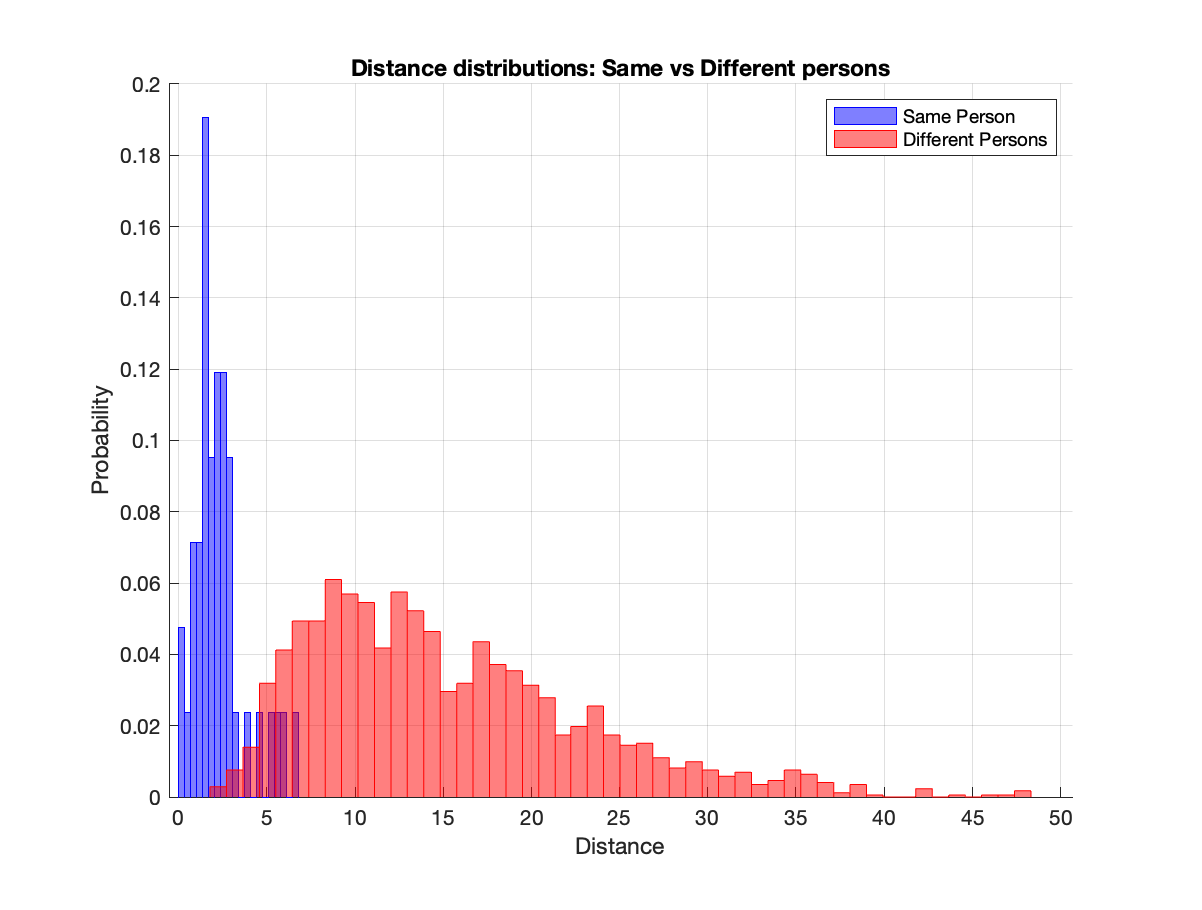
\includegraphics[width=0.75\textwidth]{figures/histograms.eps}
    \caption{Histogram of distances: Genuine (blue) vs. Impostor (red)}
    \label{fig:histograms}
\end{figure}

\subsection{FRR and FAR vs. Threshold}

The threshold $\mathrm{Th}$ defines the boundary for accepting or rejecting a verification:
\begin{itemize}[noitemsep]
    \item \textbf{False Rejection Rate (FRR)}: \( \text{FRR} = \frac{\texttt{sum(ShDist > Th)}}{\texttt{numel(ShDist)}} \)
    \item \textbf{False Acceptance Rate (FAR)}: \( \text{FAR} = \frac{\texttt{sum(OhDist $\le$ Th)}}{\texttt{numel(OhDist)}} \)
\end{itemize}

\noindent
We evaluated both metrics for 200 evenly spaced thresholds between 0 and 15.

The result is plotted in \autoref{fig:frr_far_curve}:

\begin{figure}[H]
    \centering
    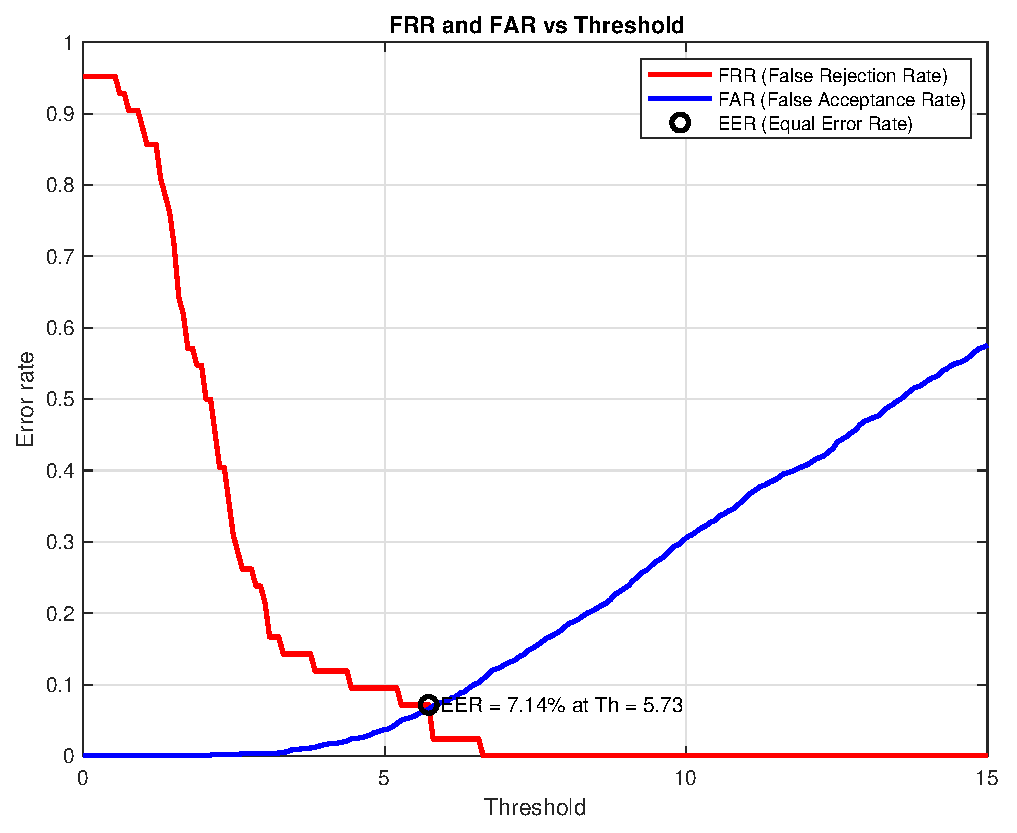
\includegraphics[width=0.75\textwidth]{figures/eer_plot.eps}
    \caption{FRR and FAR as function of threshold. The intersection defines the Equal Error Rate (EER).}
    \label{fig:frr_far_curve}
\end{figure}

\vspace{0.5em}
\noindent
\textbf{EER (Equal Error Rate)}: The error rates intersect at
\[
\text{Threshold} \approx \SI{5.73}{}, \quad \text{EER} \approx \SI{7.14}{\percent}
\]

This represents the operating point where FRR and FAR are balanced.

\subsection{Raw FRR and FAR Data (Excerpt)}

\begin{multicols}{2}
\begin{table}[H]
\centering
\caption{FRR for selected thresholds}
\begin{tabular}{@{}rrr@{}}
\toprule
Th & FR\# & FRR \\
\midrule
0.00 & 40 & 0.952 \\
0.60 & 39 & 0.929 \\
0.98 & 37 & 0.881 \\
1.73 & 24 & 0.571 \\
2.86 & 10 & 0.238 \\
3.84 & 5  & 0.119 \\
4.45 & 4  & 0.095 \\
5.28 & 3  & 0.071 \\
5.80 & 1  & 0.024 \\
6.63 & 0  & 0.000 \\
\bottomrule
\end{tabular}
\end{table}

\columnbreak

\begin{table}[H]
\centering
\caption{FAR for selected thresholds}
\begin{tabular}{@{}rrr@{}}
\toprule
Th & FA\# & FAR \\
\midrule
2.11 & 2   & 0.001 \\
2.64 & 5   & 0.003 \\
3.24 & 7   & 0.004 \\
3.92 & 24  & 0.014 \\
4.90 & 59  & 0.034 \\
5.65 & 107 & 0.062 \\
6.63 & 186 & 0.108 \\
7.84 & 295 & 0.171 \\
9.12 & 423 & 0.246 \\
11.68 & 683 & 0.397 \\
\bottomrule
\end{tabular}
\end{table}
\end{multicols}

\noindent\textbf{Summary of key MATLAB commands:}
\begin{itemize}
    \item FR errors: \texttt{sum(ShDist > Th)}
    \item FA errors: \texttt{sum(OhDist <= Th)}
    \item FRR (Slh): \texttt{FRR = sum(ShDist > Th) / numel(ShDist)}
    \item FAR (Slh): \texttt{FAR = sum(OhDist <= Th) / numel(OhDist)}
\end{itemize}

\subsection{Threshold Recommendations}

We evaluated two operational scenarios based on system requirements:

\begin{enumerate}[label=\textbf{\arabic*)}, itemsep=0.8em]
    \item \textbf{High Security (minimize FAR)} \\
    \quad Choose lowest threshold with FAR $\leq 1\%$:
    \[
    \text{Th} = \SI{3.32}{}, \quad \text{FAR} \approx \SI{0.46}{\percent}, \quad \text{FRR} \approx \SI{14.29}{\percent}
    \]

    \item \textbf{High Convenience (minimize FRR)} \\
    \quad Choose highest threshold with FRR $\leq 1\%$:
    \[
    \text{Th} = \SI{6.63}{}, \quad \text{FAR} \approx \SI{10.8}{\percent}, \quad \text{FRR} = \SI{0.00}{\percent}
    \]
\end{enumerate}

\subsection{Conclusion}

This verification analysis illustrates the trade-off between false rejections and false acceptances. The EER at $\approx$5.73 balances both, but practical deployments must select a threshold based on the system's intended use case: high-security or high-convenience.

% Section 5 – Discussion
\section{Discussion}
The system performed well for convenience-based applications, with a high TPIR(3) and low EER. However, for high-security scenarios, hand geometry alone may be insufficient due to moderate FAR. Consistency in hand measurement greatly affects system performance. Improvements could include additional features (e.g. finger contours) or multimodal fusion with fingerprint or face data.

\end{document}